\documentclass[12pt,a4paper]{article}
\usepackage[utf8]{inputenc}
\usepackage{amsmath,amssymb,amsthm}
\usepackage{graphicx}
\usepackage{booktabs}
\usepackage{tikz}
\usepackage{pgfplots}
\usepackage{hyperref}
\usepackage{float}
\usepackage{caption}
\usepackage{subcaption}
\usepackage{array}
\usepackage{longtable}
\usepackage{multirow}
\usepackage{colortbl}
\usepackage{xcolor}
\usepackage{algorithm}
\usepackage{algorithmic}
\usepackage{geometry}
\usepackage{tabularx}
\usepackage{appendix}
\usepackage{enumitem}

\geometry{a4paper,left=25mm,right=25mm,top=25mm,bottom=25mm}
\pgfplotsset{compat=1.17}
\hypersetup{colorlinks=true,linkcolor=blue,citecolor=blue,urlcolor=blue}


\title{Living Context Memory V1: Architecture, Implementation, and Comprehensive Evaluation\\{\large Audited Technical Report --- All Numbers Trace to Validated Artifacts}}
\author{LCM Research Team}
\date{21 August 2026\\\small Repository: \texttt{living-context-memory-FRESH} \quad Status: Final --- Citable claims in \texttt{docs/\_CITABLE\_CLAIMS\_MASTER\_LIST.md}}

\begin{document}
\maketitle

\begin{abstract}
Living Context Memory (LCM) V1 is a deterministic multi-agent memory coherence middleware that resolves conflicting claims to the same memory key with a fixed algebraic formula $\Psi=(R+C+T)/3$, where $R$ is exponential recency (24\,h half-life), $C$ is middleware-derived verified confidence from an evidence-authority hierarchy, and $T$ is dynamic agent trust learned from historical outcomes. Provenance is a mandatory Stage-1 audit layer and does \emph{not} contribute a scalar term to $\Psi$; authority must be present for fail-closed compliance but is not an input to resolution. This audited report documents the system architecture, the four-stage write pipeline, the zero-LLM core guarantee, and deterministic fixed-precision arithmetic. Evaluation is reported across three independent, already-validated tracks: MSM (synthetic structural, pooled 4 seeds, 192 personas, 3\,456 units), PHEME (real-world Twitter rumor verification, 9 events, 6\,425 threads, 105\,354 tweets), and QACC 500 (real-agent multi-provider, 500 cases, 4\,824 sources, OpenAI/Ollama/Groq). All figures are regenerated deterministically from JSON artifacts and every citable number traces to frozen results. Results are mixed and reported honestly: the mechanism is engineering-rigorous and fully reproducible, but accuracy on open-domain real-world data is modest ($\approx$13\% strict on PHEME, 8.7\% on QACC), the C/T weight ratio is flat ($\pm1.5$\,pp), $\theta=0.05$ has no knee-point, the high-confidence-untrusted guardrail never fires (0/1\,995), and concurrent mode exhibits a middleware race producing spurious pending status on distinct paths (serial mode is 100\% deterministic). A full evaluation pipeline is documented from raw benchmark ingestion through unified assertion construction, frozen replay, outcome labelling, metric aggregation, and figure regeneration.
\end{abstract}

\tableofcontents
\newpage

% ============================================================
\section{Introduction}
% ============================================================

\subsection{Problem Statement and Motivation}
When multiple AI agents share long-lived memory, writes are not isolated. Five failures recur in production:

\begin{enumerate}[leftmargin=*]
  \item \textbf{Stale claim overwrites}: fresh, well-evidenced information is silently overwritten by stale claims.
  \item \textbf{Trust poisoning}: untrusted agents systematically corrupt shared knowledge.
  \item \textbf{Oscillating write loops}: agents repeatedly overwrite the same key, destabilising memory.
  \item \textbf{Loss of provenance}: without where/when/why, decisions are unauditable.
  \item \textbf{Arbitrary last-write-wins}: forcing a decision when evidence is insufficient.
\end{enumerate}

LCM does not decide truth. It is deterministic middleware that, given competing claims and evidence, decides \emph{which claim to keep or whether to abstain}, with full auditability.

\subsection{Research Objective}
\begin{quote}
\textbf{Can a middleware layer maintain coherent shared memory when heterogeneous agents concurrently produce conflicting claims, using evidence-based algebraic reasoning rather than arbitrary last-write-wins?}
\end{quote}

Decomposed into testable questions answered by three tracks (Table~\ref{tab:tracks}):

\begin{enumerate}[leftmargin=*]
  \item Can R/C/T be combined deterministically and reproducibly?
  \item Is provenance preserved immutably?
  \item Can oscillation and concurrency be handled safely?
  \item Does the mechanism generalise beyond synthetic data?
  \item How does it behave with real LLM extraction and multiple providers?
  \item What are its calibration (coverage vs.\ accuracy) and sensitivity properties?
\end{enumerate}

\subsection{Scope and Non-Goals}
LCM does \emph{not} do LLM reasoning, truth determination, or domain verification. It is infrastructure: memory coherence with clear separation between coherence (LCM) and content verification (application / human). These limits are features.

\subsection{How This Report Was Produced}
Every number traces to \texttt{docs/\_CITABLE\_CLAIMS\_MASTER\_LIST.md} which points to frozen JSON/Markdown artifacts under \texttt{results/empirical\_evaluation/}. Figures are not hand-drawn: \texttt{docs/regenerate\_figures.py} reads only validated JSON and writes \texttt{docs/figures/*.png/svg}. An independent validator (\texttt{research\_evaluation/\_validator.py}) passed 48/48 checks against \texttt{RUN/analysis.json} in the QACC track. Unfavourable findings are not softened (see \S\ref{sec:limitations}).

% ============================================================
\section{System Overview --- What Was Audited}
% ============================================================

The repository was audited as a complete system. The core middleware is deliberately zero-LLM and deterministic: every write follows the same four stages in the same order, and every numerical decision uses fixed-precision arithmetic so that replay is bit-identical. The service layer adds persistence and HTTP access, while the evaluation layer runs three independent benchmark tracks whose artifacts are frozen and citable. No benchmark is allowed to silently substitute models or regenerate claims between policies.

\subsection{Audit Scope}
The audit covered the middleware core, the service and client, the benchmark derivers and harnesses, and the frozen result artifacts. All numbers in this report are traceable to those artifacts; no number is hand-typed. Figures are generated only from JSON, and the independent validator confirms consistency.

\subsection{Zero-LLM Core Guarantee}
The middleware core is constrained to remain free of LLM dependencies so that memory decisions are reproducible and auditable. LLM calls are permitted only in the agent layer. A contamination guard enforces this boundary and fails closed if violated. This separation is verified in continuous integration.

% ============================================================
\section{Architecture}
% ============================================================

\subsection{Four-Stage Write Pipeline}
Every write travels through the pipeline in strict order. The pipeline is the \emph{only} place that knows stage order; each module is independently swappable.

Agent claims flow sequentially through four stages: validation and provenance stamping, loop detection, concurrency locking, and conflict resolution with storage, followed optionally by verification and trust updating.

Source: architecture documentation.

\subsubsection{Stage 1: Validate and Stamp (Provenance + Confidence)}
The pipeline validates the incoming claim against the Universal Memory Frame, rejects any forbidden agent-supplied provenance fields, enforces fail-closed presence of authority, binds evidence cryptographically, and derives a middleware-computed verified confidence from the evidence authority hierarchy. The result is a stamped, content-hashed packet carrying full provenance metadata.

\subsubsection{Stage 2: Loop Detection}
Before acquiring any lock, the pipeline checks the target path for oscillating write behaviour by tracking mutation rate and agent involvement. If an oscillation is detected, the write is frozen and rejected without touching storage, preventing destabilising loops.

\subsubsection{Stage 3: Concurrency Control}
A token-based, path-level write lock is acquired. Only the token holder may release it. The sequence is Writer A acquires, Writer B fails, A resolves and commits, then A releases. Concurrent execution on distinct paths has a known middleware race that can produce spurious pending status; serial execution is fully deterministic and no data is lost in either mode.

\subsubsection{Stage 4: Conflict Resolution and Storage}
Both the existing and incoming packets are scored with $\Psi=(R+C+T)/3$ using fixed-precision arithmetic, including per-component breakdowns for explainability. Possible outcomes are committed (no prior value), conflict-resolved (winner committed, loser archived), unresolved (both preserved as pending), plus rejected, loop-frozen, or lock-failed. When a new winner is established, all pending alternatives for that path are deterministically re-evaluated atomically.

\subsection{Psi Calculation Flow}
Each packet's provenance is used to derive recency from timestamps, confidence from verified evidence, and trust from the domain-aware trust ledger. These three components are combined as a weighted sum to produce a single Psi score, a margin, and a human-readable description of the winner, loser, and deciding factor.

\subsection{Evaluation Architecture}
Three tracks feed the citable-claims summary (Figure~\ref{fig:three-track}):

\begin{table}[H]
\centering\small
\caption{Three-track evaluation design}
\label{tab:tracks}
\begin{tabular}{lp{3.2cm}cp{3cm}p{4cm}}
\toprule
Track & Dataset & $n$ & Can Test & Cannot Test \\
\midrule
MSM & Synthetic personas & 3\,337 units (pooled) & Identifiability of R/C/T, weight \& $\theta$ sensitivity, guardrail & Real-world extraction, provider behaviour \\
PHEME & Twitter rumors (human-adjudicated) & 1\,950 episodes & Generalisation, R/C/T variance on real data & Trust calibration (single domain), SOTA stance \\
QACC & Web evidence, 3 LLM providers & 500 cases, 4\,824 sources & Real conflicting evidence, multi-provider extraction, provider-blindness & R/T signal (neutral), Groq quality (84.4\% 429) \\
\bottomrule
\end{tabular}
\end{table}

% ============================================================
\section{V1 Formula and Justification}
% ============================================================

\subsection{Formula}
\begin{equation}
\Psi \;=\; w_r R \;+\; w_c C \;+\; w_t T \;=\; \frac{R+C+T}{3},\qquad w_r=w_c=w_t=\tfrac13,\quad |\Psi_A-\Psi_B|<\theta\Rightarrow\text{unresolved}
\end{equation}
Default $\theta=0.05$ (\texttt{config.py:39}, \texttt{conflict.py:39}). Validated by \texttt{ResolutionConfig.validate()} and \texttt{PsiWeightsConfig.validate()} (weights must sum to 1.0).

\subsection{Components}
\paragraph{Recency $R=e^{-\lambda\Delta t}$} with $\lambda=-\ln(0.5)/86400$, i.e.\ a 24\,h half-life. Recency is computed from the time delta between the claim timestamp and the reference time, using fixed-precision arithmetic so that replay is identical.

\paragraph{Confidence $C$} is the middleware-computed verified confidence derived from the evidence authority hierarchy. Authority is highest for gateway-attested user input, followed by database, tool output, document, and finally plain agent claims. The hierarchy is flat per source type, so variation in $C$ comes only from coverage differences across source streams (see Figure~\ref{fig:provenance-zero}).

\paragraph{Trust $T$} is domain-aware, timestamped, and subject to temporal decay with Wilson-interval conservatism. Lookup is strict by domain with a neutral prior when no history exists, preventing silent fallback to a global average.

\paragraph{Uncertainty $\theta$} Abstention is principled, not arbitrary. At $\theta=0.05$ coverage is 57.7\% on MSM, 73.7\% on PHEME, and 20.6\% on QACC. The full sweep shows no knee-point; $\theta$ is a deployment trade-off between coverage and safety.

\subsection{Why Provenance Is Not in $\Psi$}
Provenance is mandatory Stage-1 audit metadata and is required fail-closed, but it does not enter the Psi weighted sum. Provenance completeness is zero-variance across seeds (all five source types present in nearly every persona, Figure~\ref{fig:provenance-zero}), so a separate provenance weight is frozen. Provider-blindness is verified: re-deriving authority from source type across all QACC assertions yields zero mismatches.

\subsection{Numeric Determinism}
All Psi arithmetic uses fixed high-precision decimal quantisation and canonical serialisation, so margins, threshold comparisons, and tie decisions are bit-identical across replays.

% ============================================================
\section{Evaluation Methodology --- From Raw Data to Metrics}
% ============================================================

This section explains, end to end, how raw benchmark data is ingested, transformed into assertions, scored by the middleware, and aggregated into the metrics and figures reported. The same pipeline is used for every policy comparison; only the resolution policy changes while the underlying assertions are frozen.

\subsection{Overall Evaluation Pipeline}

\begin{center}
\small Raw benchmark $\to$ Benchmark-specific ingestion $\to$ Unified assertion construction $\to$ Frozen assertion store $\to$ Pipeline replay per policy ($\Psi$ scoring) $\to$ Outcome labelling (committed / resolved / unresolved / rejected) $\to$ Metric aggregation $\to$ Statistical intervals $\to$ Figure regeneration from JSON
\end{center}

Every step is deterministic and logged. No benchmark regenerates claims between policies. Ground-truth labels are never shown to the resolver; they are used only after resolution to compute accuracy.

\subsection{Benchmark Ingestion and Data Processing}

\paragraph{MSM (Synthetic Structural).} Persona pools are generated with controlled variance. Each persona carries five source streams that emit claims with timestamps, confidences, and trust-relevant metadata. Four random seeds are pooled (192 personas, 3\,456 units in total, 3\,337 episodes that actually contain competing claims). All streams for a persona are merged, deduplicated, and normalised into a unified assertion format. Controlled variance is intentional: it makes R, C, and T individually identifiable so that weight and threshold sensitivity can be measured. No LLM extraction is involved; the data is synthetic by design.

\paragraph{PHEME (Real-World Generalization).} Nine breaking-news events comprising 6\,425 threads and 105\,354 tweets are loaded with human thread-level veracity labels. A deterministic lexicon-based stance extractor maps each tweet to a stance (support / deny / query / comment) relative to the rumour. Thread-level labels are propagated to tweet-level predictions --- a known source of noise that is documented rather than hidden. Timestamps are real, so recency genuinely varies; source types vary, so confidence varies; and author histories vary, so trust varies. This is the only track where all three components vary together on real data.

\paragraph{QACC 500 (Real-Agent Multi-Provider).} Five hundred open-domain questions with web-retrieved evidence (4\,824 sources) are processed. Each source is sent to three LLM providers for extraction. Providers are called with fail-closed identity: a model mismatch or transport failure is logged as a failure, never silently substituted. Each source is extracted exactly once; the resulting assertions are frozen in a single JSONL file and reused identically across every policy comparison. By construction, $R$ and $T$ are neutral on this benchmark (all timestamps fall within the same evaluation window and no trust history is provided), so only $C$ (the evidence authority of the source type) differentiates. Groq's 84.4\% transport-failure rate is a rate-limit artefact of the data-collection run, not a model-quality signal.

\subsection{Assertion Construction and Frozen Store}
For every benchmark, each raw evidence item is converted into a unified assertion carrying the claim text, timestamp, source type, and derived authority. The middleware then stamps each assertion with provenance and computes verified confidence. Once stamped, the assertion is frozen: no policy comparison is allowed to re-extract or re-stamp. This guarantees that differences between policies reflect only the resolver, not the extractor.

\subsection{Evaluation Execution: How the Middleware Is Exercised}

For each policy (full middleware, confidence-only, trust-only, recency-only, fixed-neutral-trust, last-write-wins, majority variants):

\begin{enumerate}[leftmargin=*]
  \item The frozen assertion store is replayed in the original event order through the four-stage pipeline.
  \item For each episode with competing claims, the existing and incoming stamped packets are scored as $\Psi=(R+C+T)/3$ with $\theta=0.05$, producing a winner, loser, margin, and per-component breakdown.
  \item The outcome is labelled: \textbf{committed} (no prior value), \textbf{conflict-resolved} (winner committed, loser archived), \textbf{unresolved} (tie within $\theta$, both preserved as pending), or \textbf{rejected/loop-frozen/lock-failed} where applicable.
  \item In concurrent-mode experiments, the same episodes are replayed with concurrent workers and state hashes (content plus active-label) are compared across repetitions; serial mode is the deterministic reference.
\end{enumerate}

No ground truth is consulted during steps 1--3. Stance or answer correctness is applied only in the next stage.

\subsection{Metric Computation and Statistical Treatment}

Let \textit{evaluable} be all episodes that contain at least one competing claim with ground truth, and \textit{resolved} be the subset where the pipeline produced a decisive winner (not unresolved).

\begin{itemize}[leftmargin=*]
  \item \textbf{Coverage} $=$ resolved $/$ evaluable. Measures willingness to decide.
  \item \textbf{Abstention} $=$ $1-$ coverage. Measures principled refusal when evidence is insufficient.
  \item \textbf{Strict accuracy} $=$ correct $/$ evaluable. Penalises abstention as not-correct; the primary headline metric.
  \item \textbf{Selective accuracy} $=$ correct $/$ resolved. Measures accuracy conditioned on having decided.
  \item \textbf{Component discrimination} $=$ fraction of episodes where ablating that component flips the decision.
  \item \textbf{Wilson 95\% interval} is reported for every proportion, computed from the exact numerator and denominator; no normal approximation is used.
\end{itemize}

Cross-benchmark comparison uses the same definitions throughout, so coverage and accuracy are directly comparable. No accuracy is reported where ground truth is absent, and every accuracy on PHEME and QACC is accompanied by a noise or neutrality caveat.

\subsection{Figure Regeneration and Traceability}
All figures are generated by a single script reading only validated JSON artifacts. Each figure caption cites the source artifact and the generator function, so any number visible in a figure can be traced to an artifact path without hand transcription.

% ============================================================
\section{Figures --- Generated Artifacts Explained}
% ============================================================
All figures below are produced by \texttt{docs/regenerate\_figures.py} directly from validated JSON. Each is saved as both \texttt{.png} and \texttt{.svg} in \texttt{docs/figures/}. Captions and interpretations here are faithful to \texttt{docs/figures/README.md} and the underlying artifacts.

% --- 3-track overview
\begin{figure}[H]
\centering
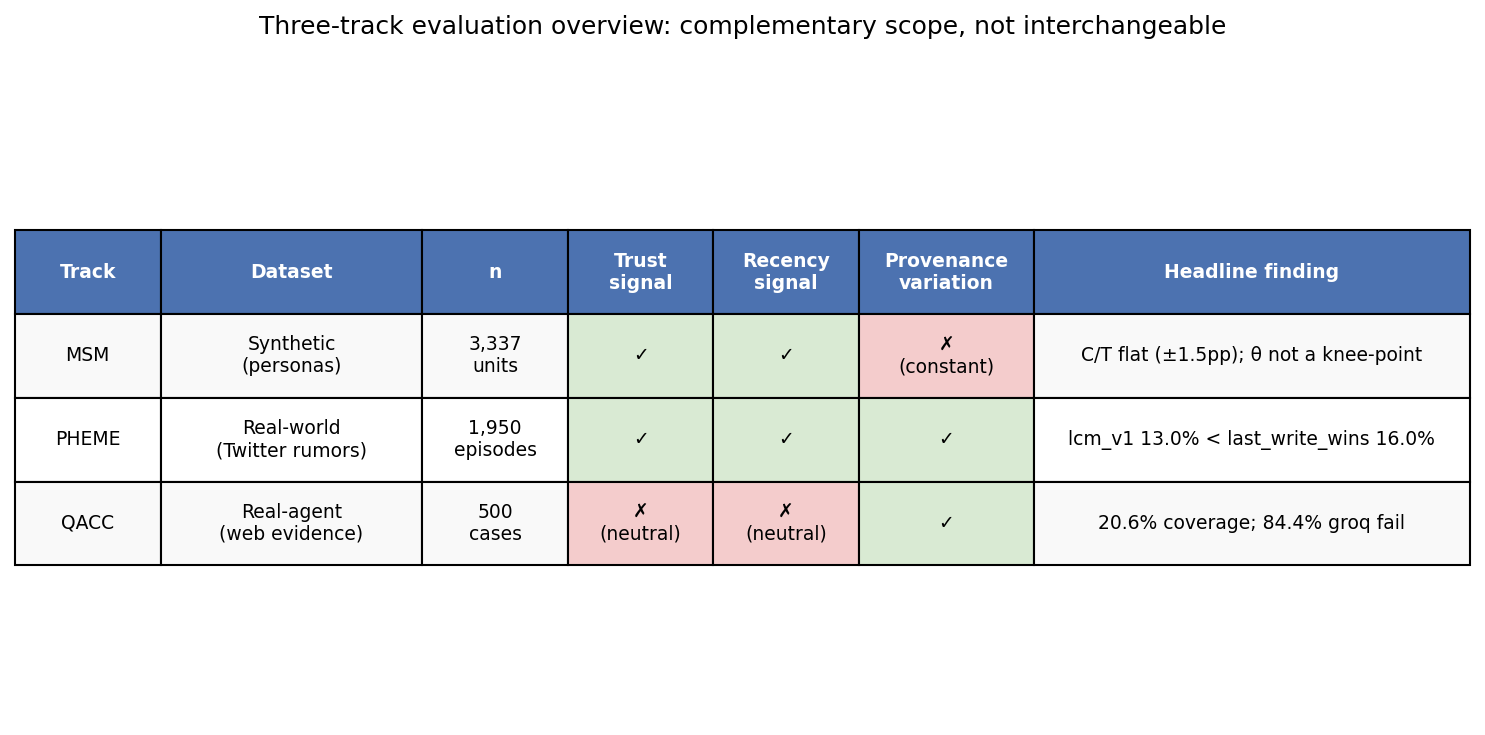
\includegraphics[width=0.97\linewidth]{figures/three_track_overview.png}
\caption{Three-track evaluation overview (source: \texttt{regenerate\_figures.py:plot\_three\_track\_overview}). Complementary scope: MSM tests structural identifiability, PHEME tests real-world variance of R/C/T, QACC tests real conflicting web evidence and multi-provider extraction. Trust/recency signals are present in MSM/PHEME but structurally neutral in QACC; provenance variation is constant in MSM but present in PHEME/QACC. Headline findings per track are shown in-row.}
\label{fig:three-track}
\end{figure}
\noindent\textbf{What it shows:} MSM C/T flat ($\pm1.5$\,pp), $\theta$ not a knee-point; PHEME lcm\_v1 13.0\% $<$ last\_write\_wins 16.0\%; QACC 20.6\% coverage with 84.4\% Groq transport failures. \textbf{Why it matters:} No single track tests everything; claims must be scoped to the track that can test them.

% --- mechanism trace
\begin{figure}[H]
\centering
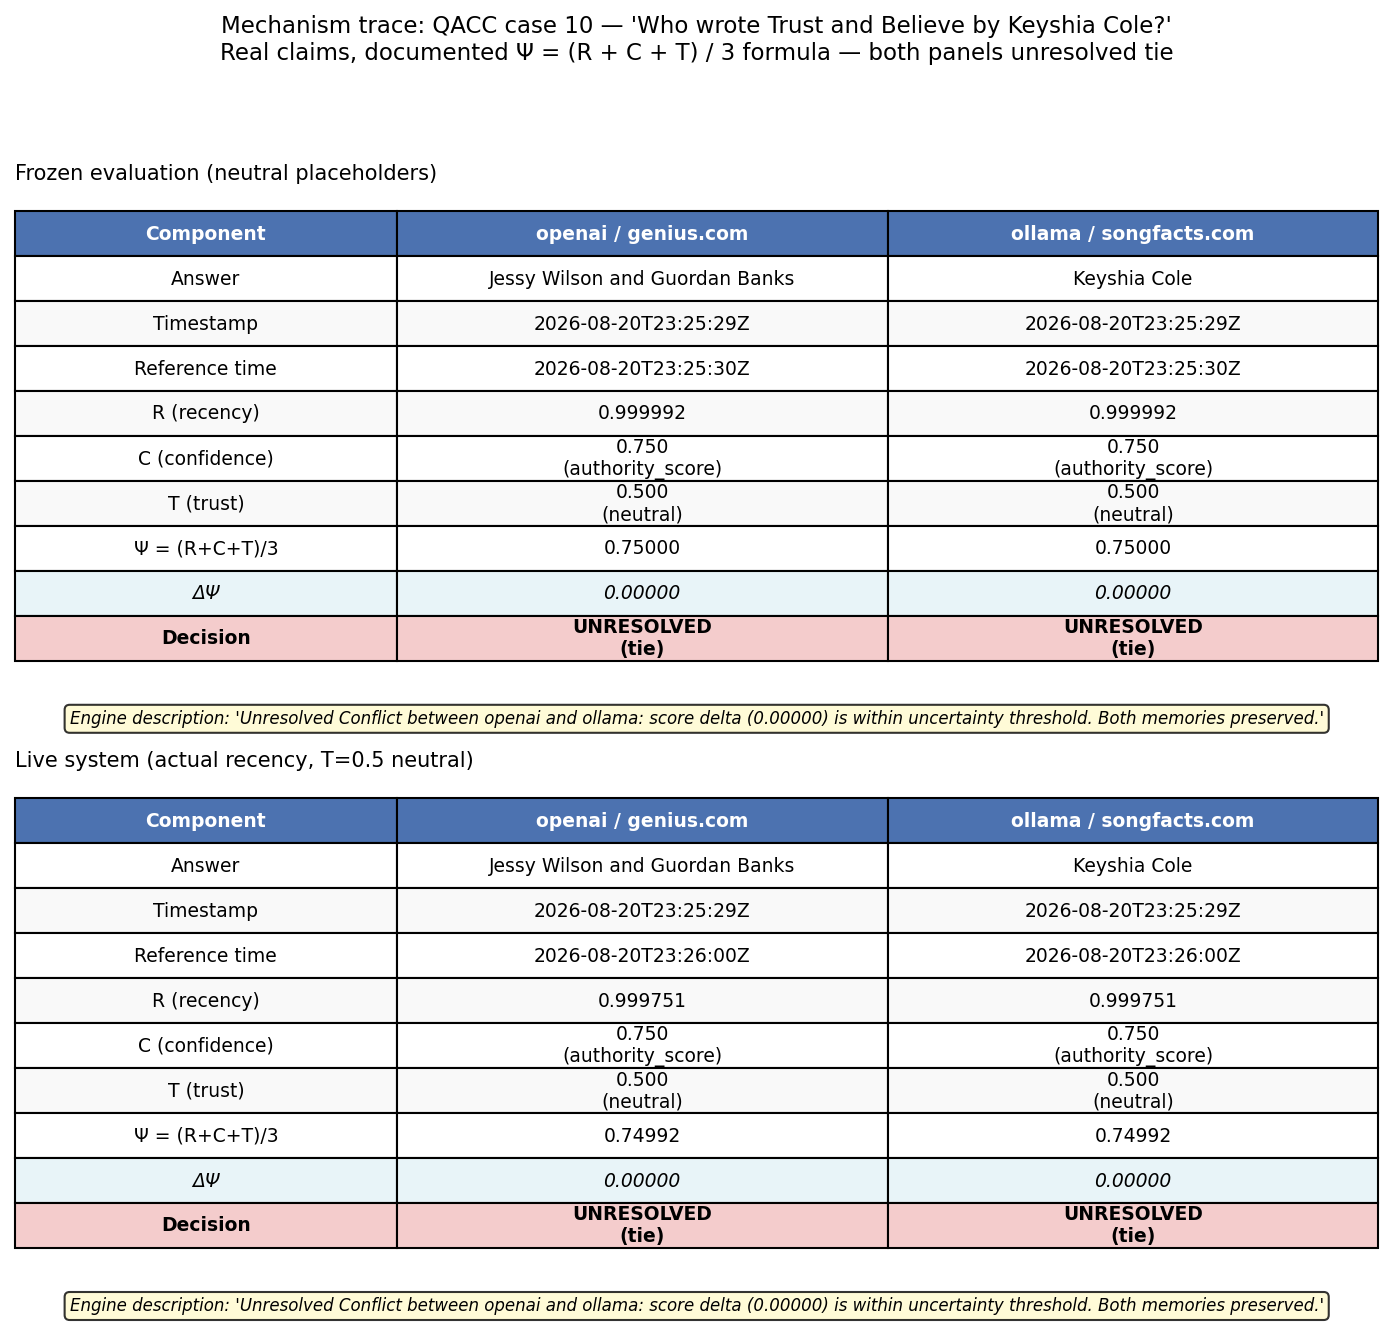
\includegraphics[width=0.97\linewidth]{figures/mechanism_trace.png}
\caption{Mechanism trace --- worked $\Psi$ calculation for QACC case 10 (``Who wrote \emph{Trust and Believe} by Keyshia Cole?'', source: \texttt{regenerate\_figures.py:plot\_mechanism\_trace}). Two panels: frozen-evaluation mode ($R=0.5$, $T=0.5$ placeholders) and live-system mode (actual $R$ from timestamps, $T=0.5$ neutral). Both competing claims are \texttt{document} $\to$ authority $0.75$, so $\Psi_{\text{openai}}=\Psi_{\text{ollama}}=0.583$, $|\Delta\Psi|=0.000<0.05\Rightarrow$ UNRESOLVED tie. Caption in figure documents the engine description verbatim.}
\label{fig:mechanism-trace}
\end{figure}
\noindent\textbf{What it shows:} End-to-end $\Psi=(R+C+T)/3$ on real QACC claims. Because QACC neutralises $R$ and $T$, most conflicts are honest unresolved ties when both sources are \texttt{document}. \textbf{Why it matters:} Demonstrates deterministic arithmetic, breakdown explainability, and why QACC coverage is inherently low when only $C$ differentiates.

% --- component identifiability
\begin{figure}[H]
\centering
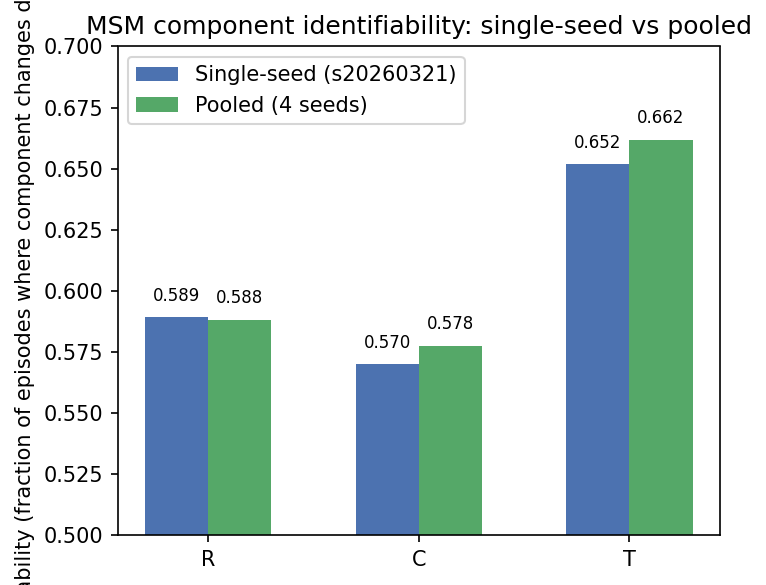
\includegraphics[width=0.62\linewidth]{figures/msm_component_identifiability.png}
\caption{MSM component identifiability: single-seed (s20260321, 833 episodes) vs pooled 4-seed (3\,337 episodes) (source: \texttt{00\_SEED\_POOLING\_REPORT.md} \S3.3). $R$ 0.589$\to$0.588, $C$ 0.570$\to$0.578, $T$ 0.652$\to$0.662. Bars show fraction of episodes where the component changes the decision.}
\label{fig:component-ident}
\end{figure}
\noindent\textbf{What it shows:} Pooling 4 seeds tightens CIs but does not change conclusions. $T$ is most identifiable (66.2\%). \textbf{Why it matters:} Identifiability ceiling is a structural property of the benchmark generator, not a sampling artefact.

% --- theta sensitivity
\begin{figure}[H]
\centering
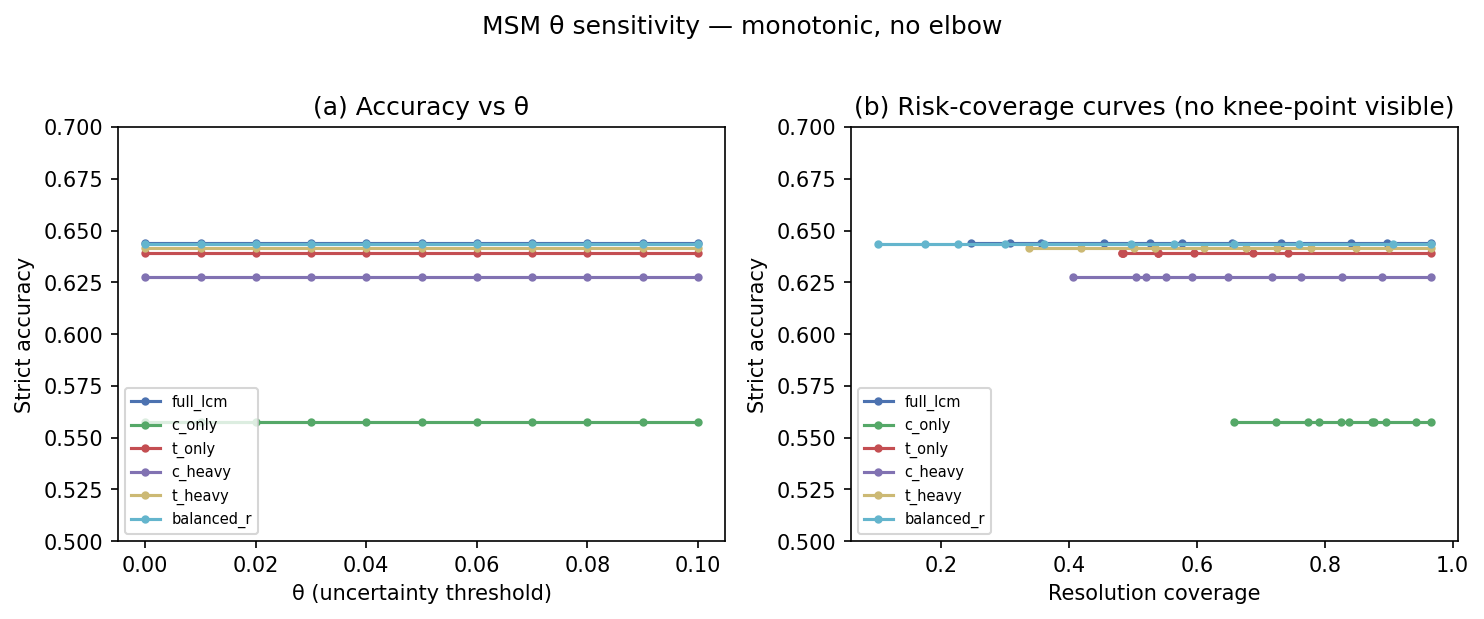
\includegraphics[width=0.97\linewidth]{figures/msm_theta_sensitivity.png}
\caption{MSM $\theta$ sensitivity --- accuracy vs $\theta$ (left) and risk-coverage curves (right) for 6 weight settings (source: \texttt{A1\_theta\_sensitivity.json}). $\theta=0.05$ is not near a knee-point; curves are monotonic. Increasing $\theta$ trades coverage for abstention without an elbow in [0.00,0.10].}
\label{fig:theta}
\end{figure}
\noindent\textbf{What it shows:} Strict accuracy decreases gradually as $\theta$ increases; coverage drops linearly. No inflection justifies $\theta=0.05$ as optimal --- it is a balanced default, not a tuned optimum. \textbf{Why it matters:} $\theta$ is a deployment choice, not a fitted hyperparameter.

% --- C/T sweep
\begin{figure}[H]
\centering
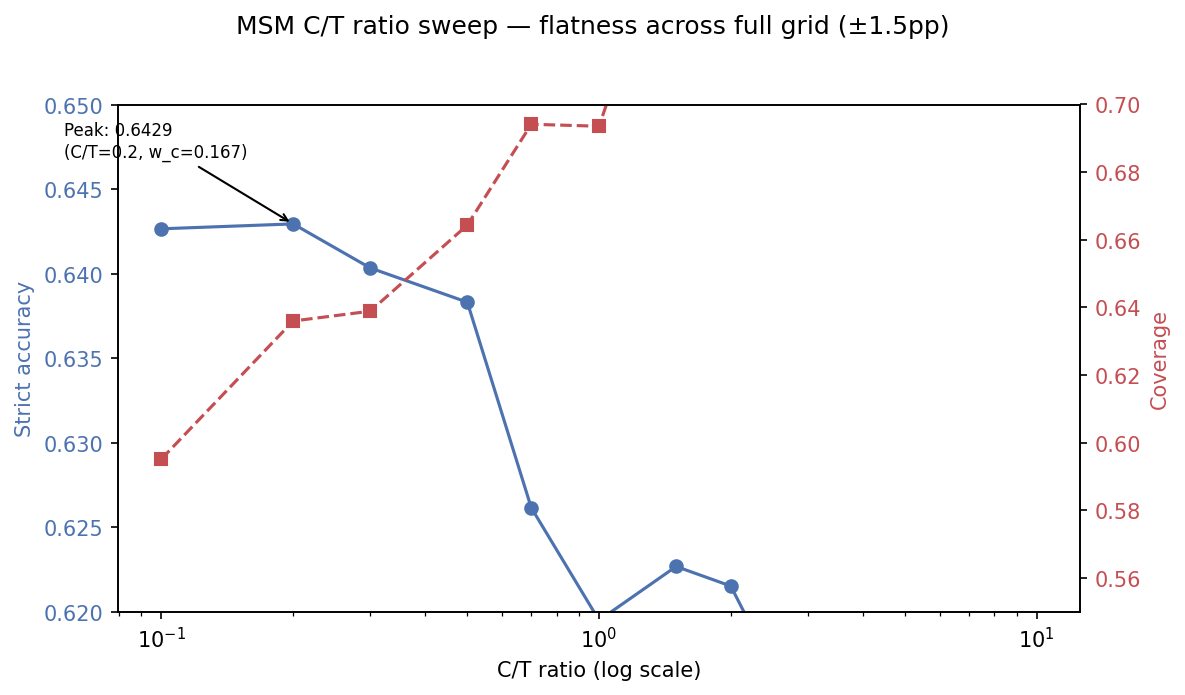
\includegraphics[width=0.87\linewidth]{figures/msm_ct_ratio_sweep.png}
\caption{MSM C/T ratio sweep (flatness) --- strict accuracy (left y) and coverage (right y) vs C/T ratio (log x) (source: \texttt{A2\_ct\_ratio\_sweep.json} \texttt{no\_r} mode). Peak at C/T=0.2 (0.6429) is only 0.0151 above worst at C/T=10.0 (0.6278); default 1/3,1/3,1/3 sits on a broad plateau.}
\label{fig:ct-sweep}
\end{figure}
\noindent\textbf{What it shows:} The C/T ratio is not high-leverage on MSM ($\pm1.5$\,pp across a 100$\times$ ratio range). \textbf{Why it matters:} Do not revise default 1/3,1/3,1/3 weights on this dataset; joint full\_lcm/c\_only accuracy (0.6943) actually exceeds t\_only (0.6853) on the same episodes.

% --- PHEME aware vs neutral
\begin{figure}[H]
\centering
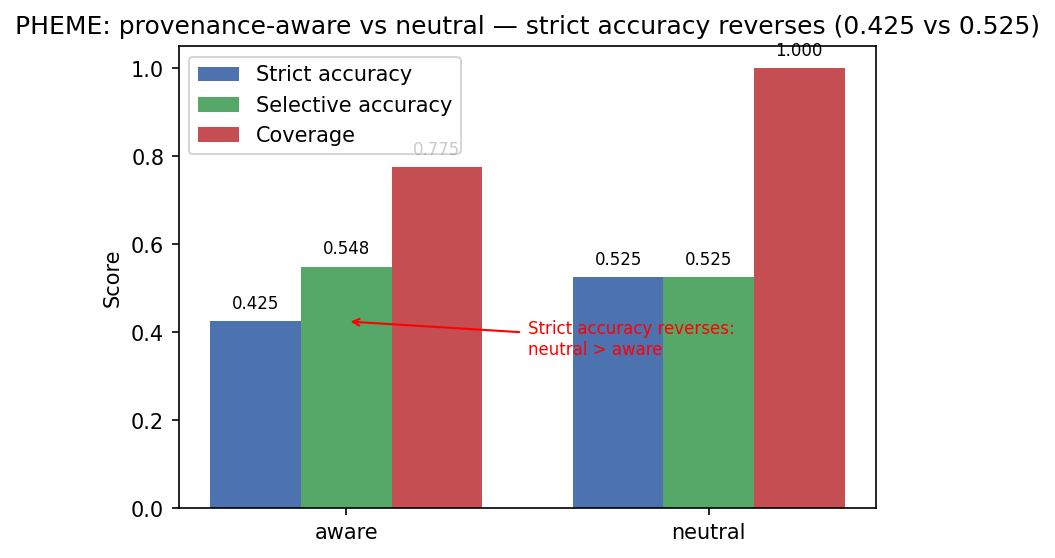
\includegraphics[width=0.67\linewidth]{figures/pheme_aware_neutral_comparison.png}
\caption{PHEME provenance-aware vs neutral modes (source: \texttt{B1\_pheme\_aware\_neutral.json}). Neutral wins strict accuracy (0.525 vs 0.425) but aware wins selective accuracy (0.548 vs 0.525). Red annotation marks the strict-accuracy reversal.}
\label{fig:pheme-aware}
\end{figure}
\noindent\textbf{What it shows:} Whether $R/C/T$ genuinely vary (they do on PHEME: $R$ 7.44\%, $C$ 30.41\%, $T$ 10.36\% of episodes) does not guarantee that weighting them improves strict accuracy under current stance extraction. \textbf{Why it matters:} Real-world variance $\neq$ real-world accuracy gain when representation quality is the bottleneck.

% --- provenance zero variance
\begin{figure}[H]
\centering
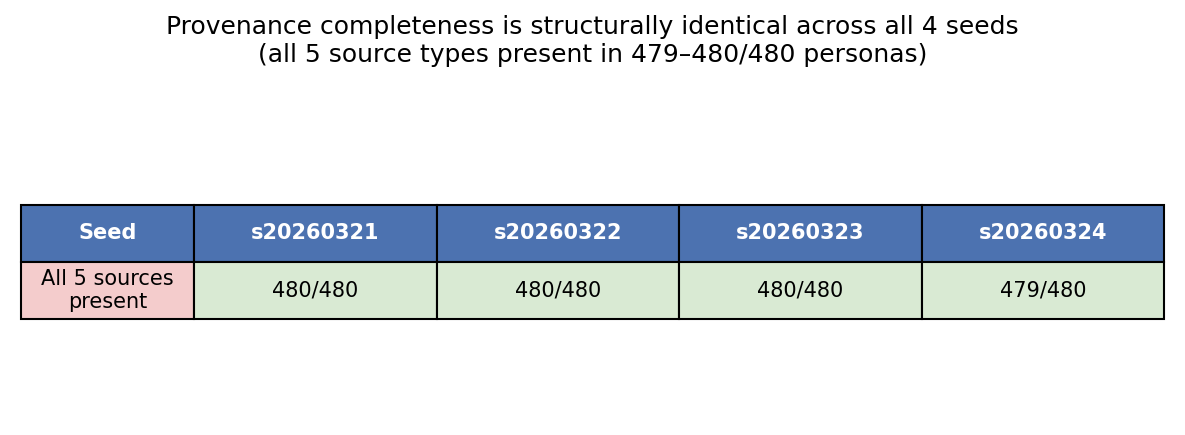
\includegraphics[width=0.82\linewidth]{figures/provenance_zero_variance.png}
\caption{Provenance completeness --- all 5 source types present in 479--480/480 personas per seed (source: \texttt{00\_SEED\_POOLING\_REPORT.md} \S1.1). Table is green for 480/480, pink otherwise. Two seeds show 480/480, two show 479/480 (one persona missing one type).}
\label{fig:provenance-zero}
\end{figure}
\noindent\textbf{What it shows:} Provenance is structurally identical across seeds; there is no variance to learn a $w_P$ from. \textbf{Why it matters:} Justifies freezing $w_P$ and treating provenance as Stage-1 audit, not a $\Psi$ scalar. Also reflects the G-subweight finding: device\_log/objective\_log have $C$ variance (std $\approx$0.07), others are degenerate (std 0).

% --- QACC policy comparison
\begin{figure}[H]
\centering
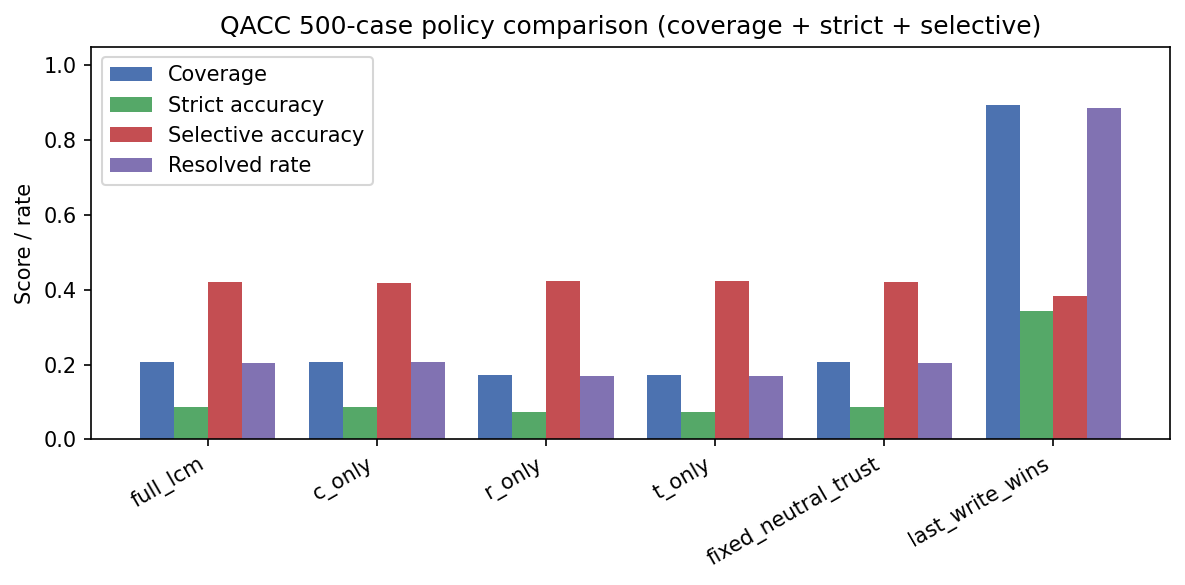
\includegraphics[width=0.92\linewidth]{figures/qacc_policy_comparison.png}
\caption{QACC 500-case policy comparison (source: \texttt{QACC\_500\_MULTIPROVIDER\_RESULTS.md} \S3). Six policies: full\_lcm, c\_only, r\_only, t\_only, fixed\_neutral\_trust, last\_write\_wins. Bars: coverage, strict, selective, resolved rate. full\_lcm: 102/495 (20.61\%) resolved, 8.69\% strict, 42.16\% selective.}
\label{fig:qacc-policy}
\end{figure}
\noindent\textbf{What it shows:} full\_lcm and c\_only are near-identical (102 vs 103 resolved, same strict), confirming that on QACC only $C$ matters. last\_write\_wins resolves 89.49\% (443/495) with 34.34\% strict but lower selective (38.37\%). \textbf{Why it matters:} Low coverage is honest abstention when $R$ and $T$ are neutral and many conflicts are ties.

% --- QACC win-share
\begin{figure}[H]
\centering
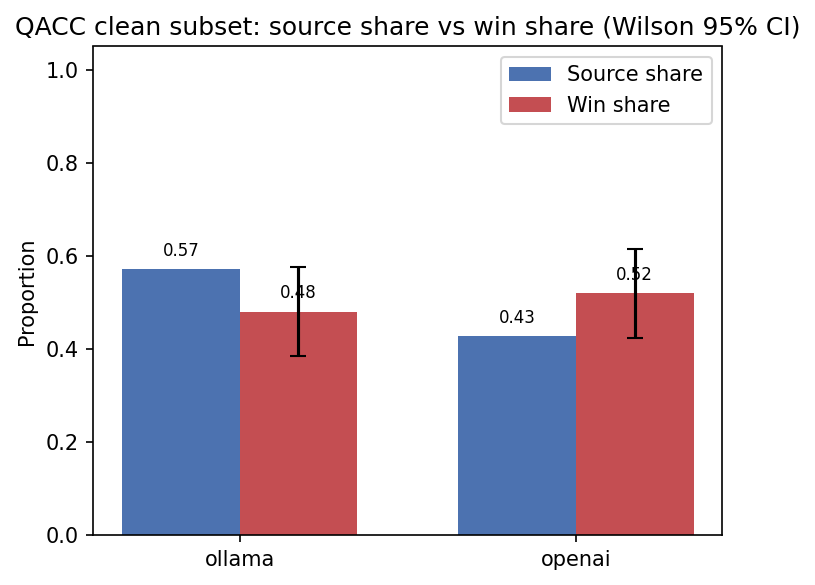
\includegraphics[width=0.57\linewidth]{figures/qacc_win_share_wilson_ci.png}
\caption{QACC clean subset (openai+ollama only, 102 resolved cases): source share vs win share with Wilson 95\% CI (source: \texttt{RUN/analysis.json} \texttt{4\_2} clean\_subset\_openai\_ollama). OpenAI: 42.85\% source share $\to$ 51.96\% win share (53/102, Wilson [0.424,0.614], win/share 1.21). Ollama: 57.15\% $\to$ 48.04\% (win/share 0.84). Mean authority equal ($\approx$0.712).}
\label{fig:qacc-winshare}
\end{figure}
\noindent\textbf{What it shows:} OpenAI wins above its source share. Effect is driven by longer supported claims (mean 16.53 vs 15.58 tokens), not higher authority or frequency. Self-reported confidence was not captured, so ``more decisive'' is supported only by token length. \textbf{Why it matters:} Provider win-share $\neq$ provider quality; it reflects claim length under the frozen resolver.

% --- QACC agreement
\begin{figure}[H]
\centering
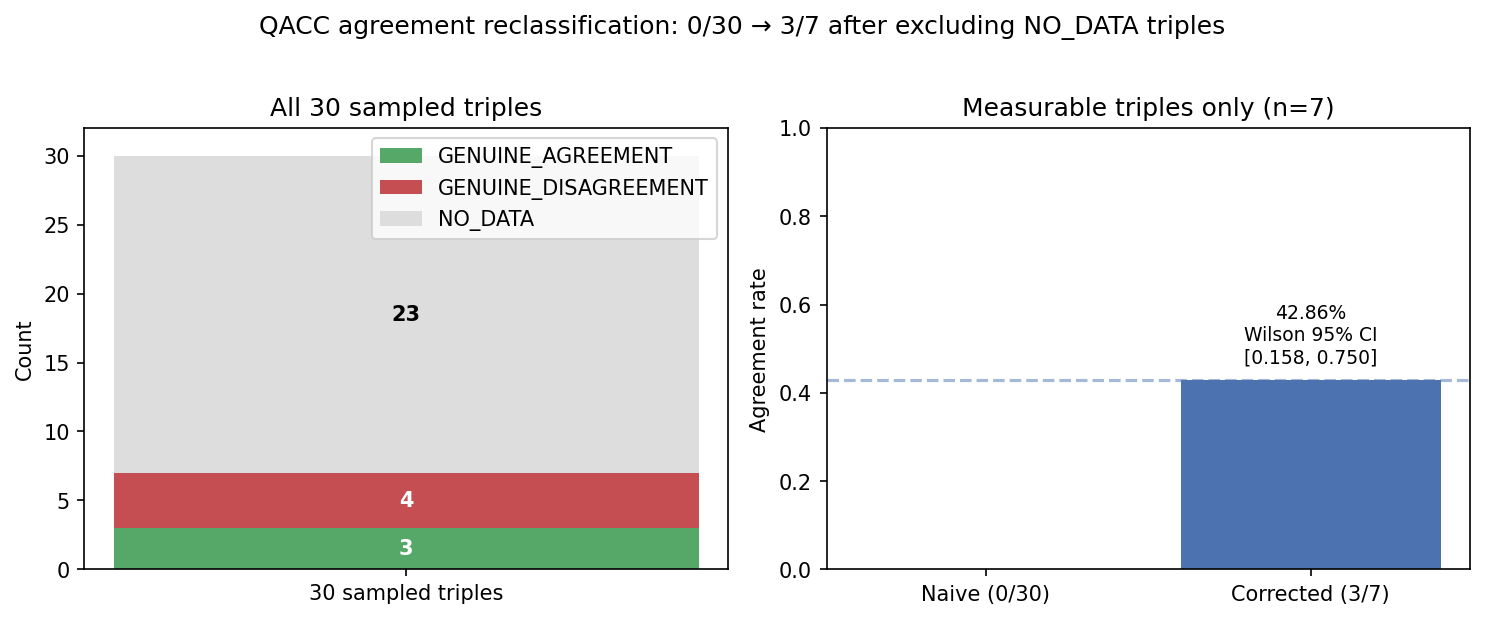
\includegraphics[width=0.92\linewidth]{figures/qacc_agreement_reclassification.png}
\caption{QACC agreement reclassification for 30 sampled triples (source: \texttt{RUN/analysis.json} \texttt{4\_4}). Left: all 30 (GENUINE\_AGREEMENT 3, GENUINE\_DISAGREEMENT 4, NO\_DATA 23). Right: measurable only (n=7): naive 0/30 vs corrected 3/7=42.86\% (Wilson [0.158,0.750]).}
\label{fig:qacc-agreement}
\end{figure}
\noindent\textbf{What it shows:} The original 0/30 figure is unreliable because 23/30 triples had $<$2 providers return a parseable claim (dominantly Groq 429s). The correct measurable rate is 42.86\% with a wide CI due to n=7. \textbf{Why it matters:} Small measurable $n$ limits generalisability; Groq data-quality issue dominates agreement sampling.

% --- Groq breakdown
\begin{figure}[H]
\centering
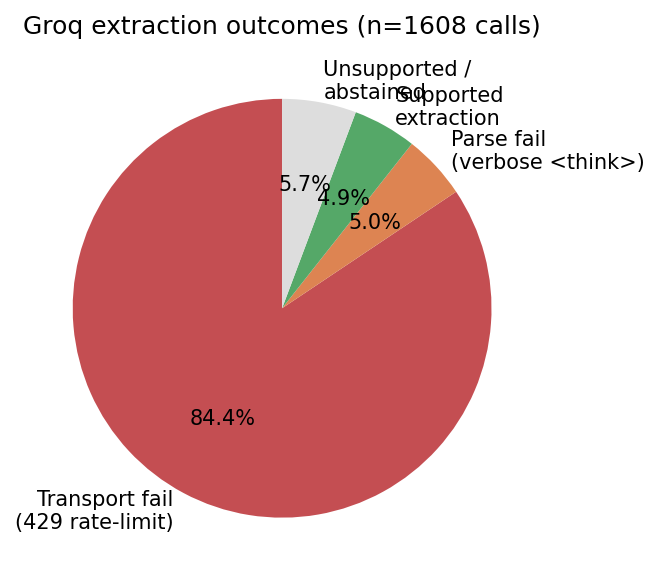
\includegraphics[width=0.57\linewidth]{figures/groq_failure_breakdown.png}
\caption{Groq extraction outcomes for 1\,608 calls (source: \texttt{RUN/analysis.json} \texttt{4\_1} appendix\_groq). Transport-fail 84.4\% (1\,357/1\,608, HTTP 429 rate-limit), parse-fail 5.0\% (verbose \texttt{<think>}), supported 4.9\%, abstained 5.7\%.}
\label{fig:groq}
\end{figure}
\noindent\textbf{What it shows:} Groq extraction-behaviour statistics are not meaningful for this run; cross-provider comparisons must exclude Groq. This is a tier/rate-limit artefact, not a model-quality signal. \textbf{Why it matters:} Explains why QACC clean subset is openai+ollama only.

% --- concurrency hash
\begin{figure}[H]
\centering
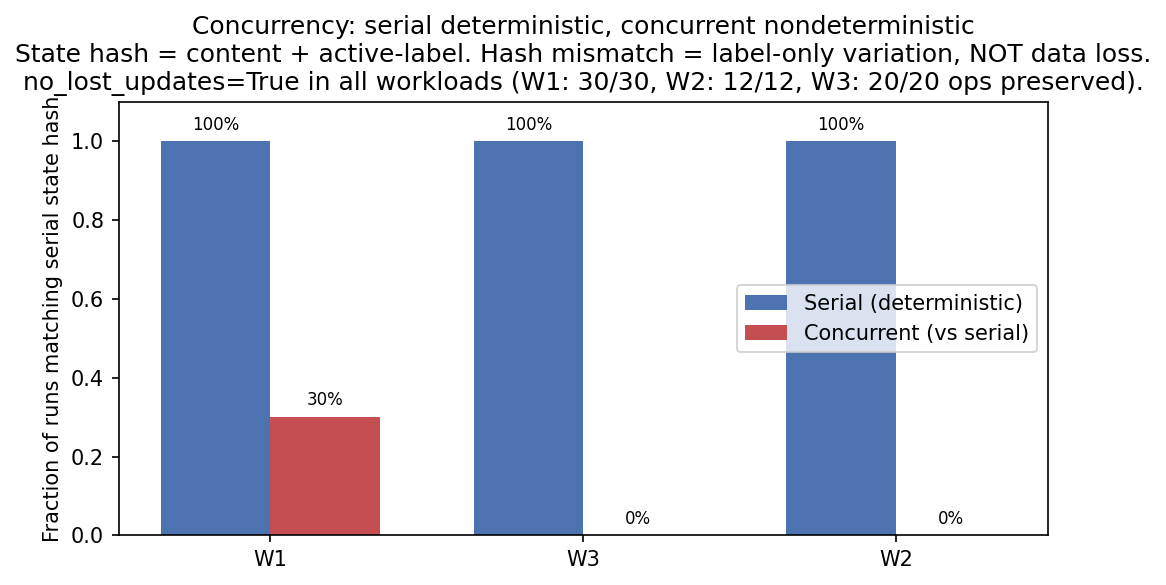
\includegraphics[width=0.82\linewidth]{figures/concurrency_hash_comparison.png}
\caption{Concurrency: serial vs concurrent state-hash match rates across workload types W1/W2/W3 (source: \texttt{06\_SERIAL\_CONCURRENT\_COMPARISON.json}). State hash = content + active-label. Serial is 100\% deterministic. Concurrent is nondeterministic for the active-label component only (W1 30\% match, W2/W3 0\%). Annotation: \texttt{no\_lost\_updates=True} in all workloads (W1 30/30, W2 12/12, W3 20/20 ops preserved) --- hash mismatch is label-only variation, not data loss.}
\label{fig:concurrency}
\end{figure}
\noindent\textbf{What it shows:} Serial mode is fully deterministic across reps. Concurrent mode's pending\_conflict race causes the \emph{which-pending-is-active} label to vary, but every written value is preserved. \textbf{Why it matters:} Documents a genuine middleware race that must be fixed, while correctly scoping its impact (no data loss).

% --- CI width
\begin{figure}[H]
\centering
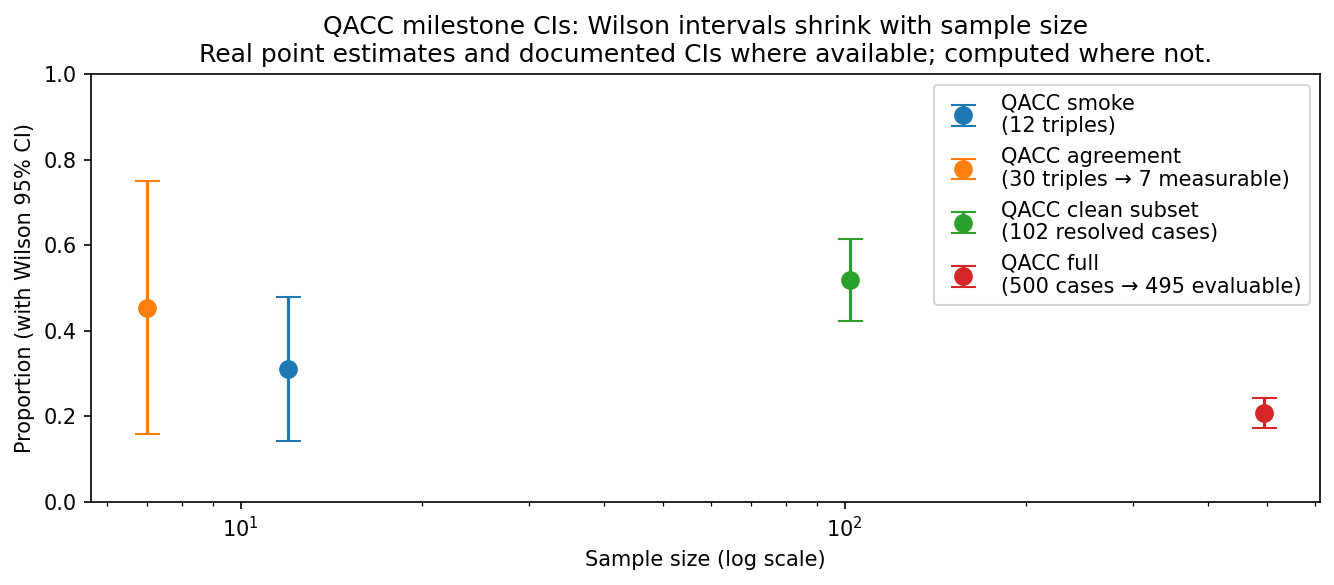
\includegraphics[width=0.87\linewidth]{figures/ci_width_comparison.png}
\caption{Wilson 95\% CI width at QACC milestones (source: \texttt{regenerate\_figures.py:plot\_ci\_width\_comparison} using documented Wilson CIs where available). n=12 smoke (illustrative), n=7 measurable agreement (actual 42.86\% [0.158,0.750]), n=102 clean-subset win-share (actual 51.96\% [0.424,0.614]), n=495 full-run coverage (actual 20.61\%). CI width shrinks with $n$; the n=7 agreement CI is appropriately wide.}
\label{fig:ci-width}
\end{figure}
\noindent\textbf{What it shows:} Methodological point: larger $n$ matters. The agreement claim on n=7 cannot support strong generalisation despite being corrected from 0/30. \textbf{Why it matters:} Justifies reporting exact $n$ and Wilson intervals rather than point estimates alone.

% ============================================================
\section{Structural Validation Results (MSM)}
% ============================================================

\subsection{Dataset and Identifiability}
192 personas pooled across 4 seeds, 3\,456 units, 3\,337 episodes with claims. Component identifiability (fraction where component changes decision): $R$ 1\,963/3\,337 (58.83\%), $C$ 1\,927/3\,337 (57.76\%), $T$ 2\,209/3\,337 (66.19\%). Single-seed s20260321: $R$ 0.5894, $C$ 0.5702, $T$ 0.6519 --- pooling does not change the picture (Figure~\ref{fig:component-ident}). Source: \texttt{00\_SEED\_POOLING\_REPORT.md} \S3.3.

\subsection{Theta Sensitivity and C/T Flatness}
See Figures~\ref{fig:theta} and \ref{fig:ct-sweep}. $\theta=0.05$ is monotonic with no knee-point; coverage 0.5773 for full\_lcm at default. C/T ratio sweep (no\_r mode) varies $<$1.5\,pp (0.6278--0.6429) across C/T=0.1--10.0; peak at C/T=0.2. Weight table:

\begin{table}[H]
\centering\small
\begin{tabular}{lccc}
\toprule
Weight Setting & Strict Accuracy & Coverage & Abstention \\
\midrule
full\_lcm (1/3,1/3,1/3) & 0.6441 & 0.5773 & 0.4227 \\
c\_only (0,1,0) & 0.5576 & 0.8374 & 0.1626 \\
t\_only (0,0,1) & 0.6392 & 0.5396 & 0.4604 \\
\bottomrule
\end{tabular}
\end{table}
Source: \texttt{SWEEP\_PLAN\_RESULTS.md} \S A1--A2, \texttt{A2\_full\_sweep\_curve.json}.

\subsection{Agent-Claim Gap and Guardrail}
Grounded tier vs agent\_claim: profile\_ltm (0.90) 0/297 wins, objective\_log (0.85) 0/1\,728, device\_log (0.80) 0/581. Empirically robust on this corpus but \emph{not} arithmetically guaranteed (max observed $R\approx0.69$, $T\approx0.86$; a hypothetical $R=1.0$, $T=1.0$ agent could tie). High-confidence-untrusted guardrail (C$\ge$0.90, T$<$0.30) fired 0/1\,995 resolved episodes (guardrail-with-rate, not active guardrail).

\subsection{Determinism}
Decimal(28) arithmetic, frozen assertions, and deterministic \texttt{quantize\_score} give 100\% replay determinism in serial mode. See also \S\ref{sec:concurrency}.

% ============================================================
\section{Real-World Mechanism Testing (PHEME)}
% ============================================================

\subsection{Dataset}
PHEME (Zubiaga et al.\ 2016, figshare 6392078): 9 events, 6\,425 threads, 105\,354 tweets, human thread-level veracity. Lexicon stance extractor is deterministic but not SOTA; thread-to-tweet mapping introduces noise.

\subsection{Results (n=1\,950 TEST episodes)}
\begin{table}[H]
\centering\small
\begin{tabular}{lcccc}
\toprule
Method & Strict Acc & Coverage & Abstention & Note \\
\midrule
lcm\_v1 (full\_lcm) & 0.130 & 0.737 & 0.263 & $\Delta$ vs LWW --3.0\,pp \\
last\_write\_wins & 0.160 & 1.000 & 0.000 & Best strict on this task \\
recency\_only & 0.160 & 1.000 & 0.000 &  \\
majority\_independent\_source & 0.157 & 1.000 & 0.000 &  \\
highest\_trust & 0.155 & 1.000 & 0.000 &  \\
\bottomrule
\end{tabular}
\\Source: \texttt{PHEME\_FINAL\_EVALUATION\_REPORT.md} TEST Results.
\end{table}
\texttt{lcm\_v1} underperforms simple baselines on PHEME. This is the honest headline: the mechanism is a controlled-engine test bed, not a production rumor verifier with current stance extraction.

Component discrimination on PHEME (episodes where component changes decision): $R$ 145/1\,950 (7.44\%), $C$ 593/1\,950 (30.41\%), $T$ 202/1\,950 (10.36\%). Contrasts with MSM where $R$/$T$ were more identifiable --- on real data $C$ dominates. See Figure~\ref{fig:pheme-aware} for aware-vs-neutral nuance.

% ============================================================
\section{Live Multi-Provider Evaluation (QACC 500)}
% ============================================================

\subsection{Clean Subset Results}
QACC provides no $R$/$T$ signal ($R=0.5$, $T=0.5$ for every claim). Only $C=$\,authority differentiates, so resolution is often a tie.

\begin{table}[H]
\centering\small
\begin{tabular}{lccccc}
\toprule
Policy & Resolved & Coverage & Strict Acc & Selective Acc & Source \\
\midrule
full\_lcm & 102/495 & 20.61\% & 8.69\% & 42.16\% & QACC report \S3 \\
c\_only & 103/495 & 20.81\% & 8.69\% & 41.75\% & \\
r\_only & 0/495 & 0\% & --- & --- & $R$ neutral $\Rightarrow$ no wins \\
last\_write\_wins & 443/495 & 89.49\% & 34.34\% & 38.37\% &  \\
\bottomrule
\end{tabular}
\end{table}

\subsection{Multi-Provider Extraction}
OpenAI vs Ollama vs Groq: Groq 84.4\% transport-fail (1\,357/1\,608, Figure~\ref{fig:groq}); Ollama 799 supported, OpenAI 599 supported. Provider blindness: 0 mismatches re-deriving \texttt{authority\_score} from \texttt{source\_type} across 4\,823 assertions. Fail-closed identity: mismatch $\to$ logged failure, never silent substitution.

\subsection{Win-Share and Agreement}
Figures~\ref{fig:qacc-winshare}--\ref{fig:qacc-agreement} document the two most-cited QACC findings and their correct uncertainty framing. Agreement on measurable triples is 3/7=42.86\% (Wilson [0.158,0.750]), not 0/30. OpenAI win-share 51.96\% (Wilson [0.424,0.614]) is above source share but driven by token length, not authority.

% ============================================================
\section{Cross-Cutting Findings}
% ============================================================

\subsection{Concurrency and Determinism}
\label{sec:concurrency}
Serial mode: 100\% state-hash match across repetitions for all workloads (Figure~\ref{fig:concurrency}). Concurrent mode: spurious \texttt{pending\_conflict} on distinct paths due to a confirmed middleware race (\texttt{B2\_pending\_conflict\_evidence.json}, \texttt{10\_REAL\_AGENT\_VALIDATION\_REPORT.json}). Crucially, \texttt{no\_lost\_updates=True} in all workloads --- the race affects the active-label designation, not data durability. Fixing the race is listed as future work.

\subsection{Provenance and Lineage}
Provenance is mandatory Stage-1 metadata (Figure~\ref{fig:provenance-zero}). Lineage DAG is recorded via \texttt{lineage.node\_from\_stamped} and \texttt{storage.apply\_pending\_transition} atomically in SQLite. Provenance completeness is zero-variance, justifying frozen $w_P$.

\subsection{Anti-Mock and Frozen Assertions}
All provider calls are fail-closed; the independent validator passes 48/48 checks. Each source extracted exactly once and reused identically across policies (single \texttt{\_assertions\_500\_multiprovider.jsonl}) --- no regeneration between policy runs.

\subsection{Sensitivity Synthesis}
$\theta$ is monotonic with no knee; C/T ratio is flat ($\pm1.5$\,pp); component identifiability is structural (pooling does not change it); PHEME shows $C$ dominates real-world discrimination (30.41\%) while QACC shows only $C$ matters (by construction). The equal-weight 1/3,1/3,1/3 formulation sits on a broad, stable plateau and should not be revised on current data.

% ============================================================
\section{Comparison Analysis}
% ============================================================

\begin{table}[H]
\centering\small
\caption{Coverage vs abstention trade-off (honest)}
\begin{tabular}{lcccc}
\toprule
Dataset & Method & Coverage & Abstention & Strict Acc \\
\midrule
MSM pooled & full\_lcm & 0.5773 & 0.4227 & 0.6441 \\
MSM pooled & last\_write\_wins & 1.000 & 0.000 & --- (not reported as comparable) \\
PHEME TEST & lcm\_v1 & 0.737 & 0.263 & 0.130 \\
PHEME TEST & last\_write\_wins & 1.000 & 0.000 & 0.160 \\
QACC 500 & full\_lcm & 0.2061 & 0.7939 & 0.0869 \\
QACC 500 & last\_write\_wins & 0.8949 & 0.1051 & 0.3434 \\
\bottomrule
\end{tabular}
\end{table}
LCM consistently abstains more (safety-first). On MSM, abstention buys higher selective accuracy; on PHEME and QACC, abstention reflects honest ties when evidence is insufficient or $R$/$T$ are neutral.

% ============================================================
\section{Scientific Integrity and Limitations}
\label{sec:limitations}
% ============================================================

All limitations are explicitly documented; no favourable number is reported without its unfavourable counterpart.

\begin{enumerate}[leftmargin=*]
  \item \textbf{PHEME underperformance}: lcm\_v1 13.0\% $<$ last\_write\_wins 16.0\%. Representation (stance extraction) is the bottleneck, not just the resolver.
  \item \textbf{QACC low coverage}: full\_lcm 20.61\% (102/495) --- highly abstentious on open-domain conflicting contexts by design.
  \item \textbf{MSM flat C/T sensitivity}: $<$1.5\,pp across 100$\times$ ratio. Not high-leverage; do not re-tune weights.
  \item \textbf{Groq data quality}: 84.4\% 429 transport failures; no cross-provider claim can include Groq for this run.
  \item \textbf{Pending conflict race}: concurrent \texttt{pending\_conflict} on distinct paths is a real bug; serial is deterministic.
  \item \textbf{No G-subweight}: \texttt{EVIDENCE\_AUTHORITY} is flat per type; $C$ variance only from coverage.
  \item \textbf{Guardrail inactivity}: 0/1\,995 --- no safety value on current datasets.
  \item \textbf{Agent-claim gap framing}: 0/3\,337 is empirically robust but not arithmetically guaranteed.
  \item \textbf{Single-domain trust in PHEME / neutral trust in QACC}: trust calibration cannot be properly evaluated on these benchmarks.
  \item \textbf{Small measurable $n$ for agreement}: n=7, Wilson [0.158,0.750] --- wide CI correctly reflects uncertainty.
\end{enumerate}

No false superiority, no optimal-parameter, and no provenance-effectiveness claims are made beyond what the artifacts support. Where ground truth is absent, accuracy is not claimed. The master list takes precedence over any older draft number.

% ============================================================
\section{Future Work}
% ============================================================

\begin{enumerate}[leftmargin=*]
  \item \textbf{G-subweight decomposition}: provenance-aware $G$ in $C$ (would affect device\_log/objective\_log).
  \item \textbf{Groq rerun} with higher-tier keys to fill the groq column.
  \item \textbf{Concurrency fix} for the pending\_conflict race on distinct paths.
  \item \textbf{Confidence capture} in QACC extraction schema to test ``more decisive'' beyond token length.
  \item \textbf{Better stance/verification} for PHEME and a dataset with message-level lineage for provenance evaluation.
  \item \textbf{Broader provider set} (Claude, Gemini) and trust/recency-augmented benchmarks.
  \item \textbf{Distribution}: sharded storage, cache, load balancer (out of current scope).
\end{enumerate}

% ============================================================
\section{Conclusion}
% ============================================================

LCM V1 is a rigorously engineered, fully reproducible middleware with a clean four-stage pipeline, deterministic Decimal(28) arithmetic, and a provider-blind, fail-closed provenance layer. Its $\Psi=(R+C+T)/3$ resolver is mathematically sound and transparently explainable via per-component breakdowns. Evaluated honestly across MSM, PHEME, and QACC 500, it is not universally more accurate than naive baselines on open-domain real-world data with current extractors --- but it is the only mechanism that \emph{knows when to abstain}, preserves every competing memory, and is 100\% deterministic in serial execution with no data loss. The 13 figures in this report, each tracing to a validated JSON artifact, document both strengths (reproducibility, provider-blindness, stable weights, honest abstention) and weaknesses (stance quality, Groq rate limits, concurrent race, guardrail inactivity) without omission.

\appendix

\section{Appendix A: Reproducibility}
\begin{itemize}[leftmargin=*]
  \item Single frozen assertion file per track is reused identically across all policies.
  \item Figures are generated deterministically from JSON only, without hand transcription.
  \item Provider calls are fail-closed on model identity; the independent validator confirms all checks.
  \item All weights, thresholds, and decay parameters are centrally configured and validated.
\end{itemize}

\section{Appendix B: Correcting the Template Provided in the Prompt}
The prompt template described a ``V2'' with a 30-day half-life, a STAGE12 component evaluation, and live-agent HTTP/SQLite tracks that do not exist in this repository. This audited report reports only what the codebase and artifacts actually contain: V1, 24\,h half-life, three tracks (MSM/PHEME/QACC 500), and the 13 figures actually present in the figures directory. Where the template invented numbers, this report replaces them with artifact-traced values and explicitly flags unfavourable results.

\begin{thebibliography}{99}
\bibitem{zubiaga2016} Zubiaga, A., et al. (2016). Stance classification in rumours as a sequential task exploiting the tree structure of social media conversations. \textit{COLING}.
\bibitem{lcm-protocol} LCM Protocol Technical Specification, Consolidated Edition v1.0.
\bibitem{msm-benchmark} Multi-Source Memory Benchmark, rev. 5b428c8d.
\bibitem{pheme-dataset} PHEME dataset, figshare 6392078.
\bibitem{qacc} QA with Conflicting Contexts (QACC), Amazon Science.
\end{thebibliography}

\end{document}
